\documentclass[]{exam}
\usepackage[utf8]{inputenc}
\usepackage{enumitem}
\usepackage{amsmath}
\usepackage{amsfonts}
\usepackage{setspace}
\usepackage{verbatim} 
\usepackage{graphicx} 
\usepackage{gensymb}
\usepackage{color}
\usepackage{commath}
\usepackage{fancyvrb}
\doublespacing
\graphicspath{C:\Users\Johnnia\Desktop\常用\Spring2017\Math 327\HW8}
\title{}

%===> Formatting ===>
\setlength{\parskip}{8pt}
\setlength{\parindent}{20pt}  
%<=== Formatting <===


\title{Math 327 HW8}
\author{Chongyi Xu}

\begin{document}
	
\maketitle
\begin{questions}
\question Show that $f:(0,1)\to\mathbb{R}$ where $f(x) = \frac{1}{x^2}$ is not uniformly continuous.
\\
\\ Let $(u_n)_{n\in\mathbb{N}} = \frac{1}{n + 1}$, $(v_n)_{n\in\mathbb{N}} = \frac{1}{(n + 1)^2}$, then $u_n - v_n \to 0$ but $f(u_n) - f(v_n) = (n + 1)^2 - (n + 1)^4 \to\infty$, which diverges. So $f$ is not uniformly continuous
\question Let $c$ be a number between 0 and 1. Without the use of Theorem 3.17, show that $f:[c, 1]\to\mathbb{R}$ where $f(x) = \frac{1}{x^2}$ is uniformly continuous. 
\\
\\ Let $f(x) = \frac{1}{x^2}:[c, 1]\to\mathbb{R}$ Let $u_n$, $v_n$ be sequence in $[c, 1]$. Assume $u_n - v_n \to 0$. Then
\begin{equation*}
\begin{split}
	\abs{f(u_n) - f(v_n)} 	&= \abs{u_n^2 - v_n^2} \\
							&= \abs{(u_n + v_n)(u_n - v_n)} \\
							&= \abs{u_n - v_n}\cdot\abs{u_n + v_n} \\
							&\leq \abs{u_n - v_n}\cdot(\abs{u_n} + \abs{v_n}) \text{(By Triangular Inequality)} \\
							&\leq \abs{u_n - v_n}\cdot(1 + 1) \text{since both $u_n$ and $v_n\in[c, 1]$)} \\
							&= 2\abs{u_n - v_n} \to 0 \text{since }u_n - v_n\to 0
\end{split}
\end{equation*}
So $\abs{f(u_n) - f(v_n)}\to 0$. Therefore, $f(x)$ is uniformly continuous.

\question Assume that $f:D\to\mathbb{R}$ and $g:D\to\mathbb{R}$ are uniformly continuous.
\begin{parts}
	\part Show by example that $fg:D\to\mathbb{R}$ does not have to be uniformly continuous.
	\\
	\\ Let $f(x) = x$, $g(x) = x$, $D = [0, \infty]$. Then both $f(x)$ and $g(x)$ are uniformly continuous but $fg = x^2$ does not.

	\part Show that if $f$ and $g$ are also bounded, then $fg:D\to\mathbb{R}$ will be uniformly continuous.
	\\
	\\ Let $f:D\to\mathbb{R}$ and $g:D\to\mathbb{R}$ be uniformly continuous and $f$, $g$ are bounded. Let $u_n, v_n$ be sequence in $D$, Assume $u_n - v_n \to 0$. Since $f$ and $g$ are bounded, assume $a_f < f(x) < b_f$ for all $x\in D$, $a_g < g(x) < b_g$ for all $x\in D$. Then
	\begin{equation*}
	\begin{split}
		\abs{f(u_n)g(u_n) - f(v_n)g(v_n)} 	&= f(u_n)[g(u_n) - g(v_n)] + g(v_n)[f(u_n) - f(v_n)] \\
											&< b_f[g(u_n - g(v_n))] + b_g[f(u_n) - f(v_n)] \text{(By construction)} \\
											&\to 0 + 0 = 0 \text{since $f$ and $g$ are uniformly continuous}
	\end{split}
	\end{equation*}
	\\ So with $f$ and $g$ bounded, $fg$ will also be uniformly continuous.

	\part Show that if $D$ is compact, then $fg:D\to\mathbb{R}$ will be uniformly continuous.
	\\ 
	\\ By Extreme Value Theorem, if $D$ is compact, $f$ and $g$ are continuous(uniformly continuous in this case), then $f$ and $g$ have max and min(bounded). So by part(b), it is proved that if $f$ and $g$ are bounded, $fg$ will be uniformly continuous.
\end{parts}

\question Determine wheter the following are true are false. If true, explain. If false, give a counter-example.
\begin{parts}
	\part A monotone function $f:\mathbb{R}\to\mathbb{R}$ is one-to-one.
	\\ It is false. Let $f$ be a constant funciton $f(x) = a,a\in\mathbb{R}\forall x\in\mathbb{R}$. In this case, $f(x_1) = f(x_2) = a$ does not necessary implies $x_1 = x_2$. So it is not one-to-one.

	\part A strictly increasing function $f:\mathbb{R}\to\mathbb{R}$ is one-to-one.
	\\ It is true. Because $f$ strictly increasing implies if $x_1 < x_2$, then $f(x_1) < f(x_2)$ by the definition. If $f(x_1) = f(x_2)$, $x_1$ and $x_2$ has to be equal.

	\part A strictly increasing function $f:\mathbb{R}\to\mathbb{R}$ is continuous.
	\\ It is false. Consider a step function
	$\begin{displaystyle}
	f(x) =
	\begin{cases}
		x, 		&\text{for } x < 1 \\
		x + 1	&\text{for } x \geq 1 \\
	\end{cases}
	\end{displaystyle}$.
	\\ In this case, $f(x)$ is strictly increasing but not continuous.

	\part A one-to-one function $f:\mathbb{R}\to\mathbb{R}$ is continuous.
	It is false. Consider a step function
	$\begin{displaystyle}
	f(x) =
	\begin{cases}
		x, 		&\text{for } x < 1 \\
		x + 1	&\text{for } x \geq 1 \\
	\end{cases}
	\end{displaystyle}$.
	\\ In this case, $f(x)$ is one-to-one but not continuous.
\end{parts}

\question For the following, a picture is ok, a formula is better, proving continuity of your function using its formula is the best.
\begin{parts}
	\part Find a continuous function $f:(0, 1)\to\mathbb{R}$ with an image equal to $\mathbb{R}$
	\\ 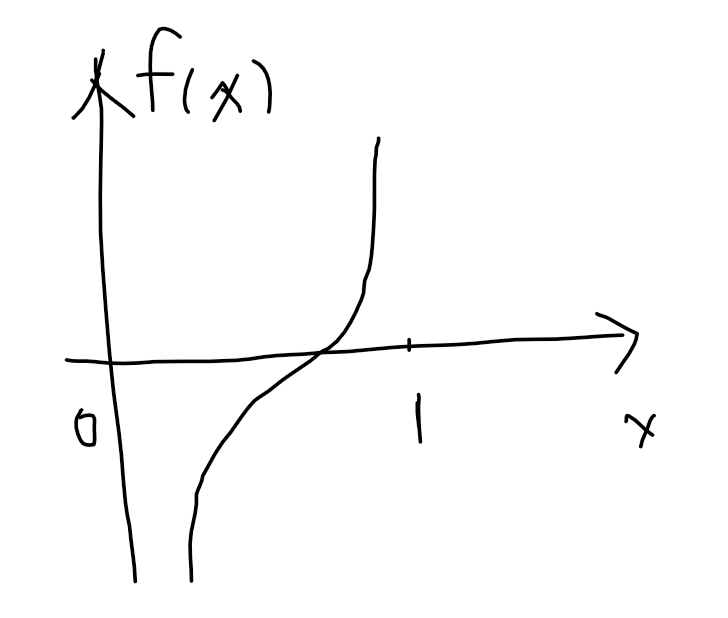
\includegraphics[scale = 0.5]{5_a.png}
	\part Find a continuous function $f:(0, 1)\to\mathbb{R}$ with an image equal to $[0, 1]$.
	\\ 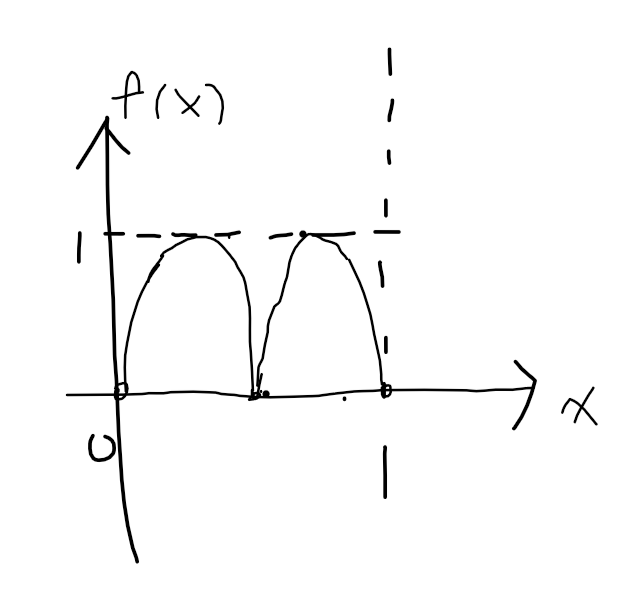
\includegraphics[scale = 0.5]{5_b.png}
	\part Find a continuous function $f:\mathbb{R}\to\mathbb{R}$ with an image equal to $(-1, 1)$
	\\ 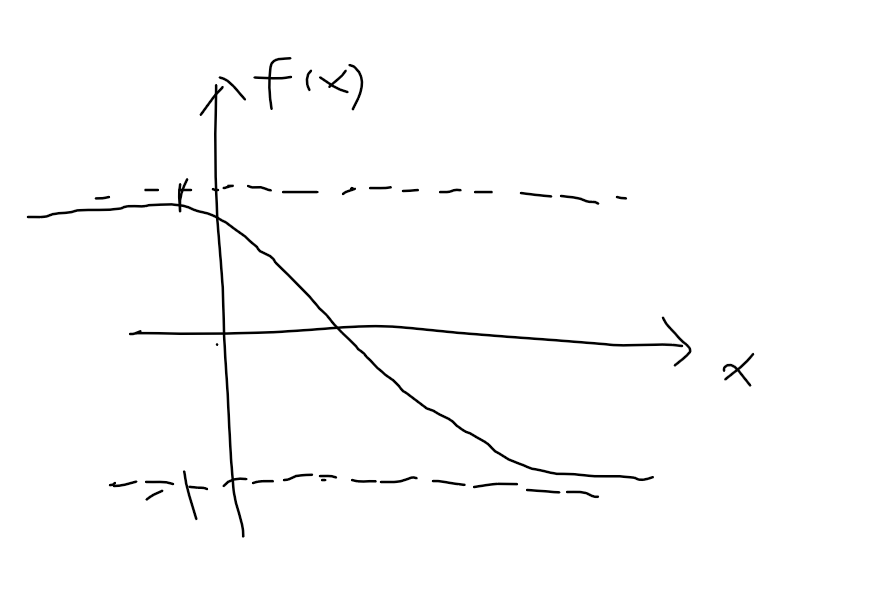
\includegraphics[scale = 0.5]{5_c.png}
\end{parts}

\question Prove that there does not exist a strictly increaisng function $f:\mathbb{Q}\to\mathbb{R}$ such that $f(\mathbb{Q}) = \mathbb{R}$.
\\
\\ Suppose $f:\mathbb{Q}\to\mathbb{R}$ is strictly increasing. Since we have proved in preivous homeworks that $\mathbb{Q}$ is not compact, then there exists a convergent sequence $(a_n)\in\mathbb{Q}$ such that $a_n\to a$ but $a\not\in\mathbb{Q}$. Since $f$ is strictly increasing, $f(a_n) < f(a)$ for all $n$. So $f(a)\in\mathbb{R}$ is not in the image of $f(\mathbb{Q})$.

\end{questions}
\end{document} 
